% This is samplepaper.tex, a sample chapter demonstrating the
% LLNCS macro package for Springer Computer Science proceedings;
% Version 2.21 of 2022/01/12
%

\documentclass[runningheads]{llncs}

\usepackage{amssymb}%
\usepackage{amsmath}
\usepackage{tikz}
\usepackage[T1]{fontenc}
% T1 fonts will be used to generate the final print and online PDFs,
% so please use T1 fonts in your manuscript whenever possible.
% Other font encondings may result in incorrect characters.
%
\usepackage{graphicx}
% Used for displaying a sample figure. If possible, figure files should
% be included in EPS format.
%
% If you use the hyperref package, please uncomment the following two lines
% to display URLs in blue roman font according to Springer's eBook style:
%\usepackage{color}
%\renewcommand\UrlFont{\color{blue}\rmfamily}
%\urlstyle{rm}
%
\begin{document}
%
\title{Contribution Title}
%
%\titlerunning{Abbreviated paper title}
% If the paper title is too long for the running head, you can set
% an abbreviated paper title here
%
\author{First Author\inst{1}\orcidID{0000-1111-2222-3333} \and
Second Author\inst{2,3}\orcidID{1111-2222-3333-4444} \and
Third Author\inst{3}\orcidID{2222--3333-4444-5555}}
%
\authorrunning{F. Author et al.}
% First names are abbreviated in the running head.
% If there are more than two authors, 'et al.' is used.
%
\institute{Princeton University, Princeton NJ 08544, USA \and
Springer Heidelberg, Tiergartenstr. 17, 69121 Heidelberg, Germany
\email{lncs@springer.com}\\
\url{http://www.springer.com/gp/computer-science/lncs} \and
ABC Institute, Rupert-Karls-University Heidelberg, Heidelberg, Germany\\
\email{\{abc,lncs\}@uni-heidelberg.de}}
%
\maketitle              % typeset the header of the contribution
%
\begin{abstract}
Tableaux proofs are used in automated  "proofers" as (TODO), whereas sequent calculus 
proofs are used in proof assistants as (TODO). This work aims to discuss the translation between them and provide an 
algorithm for translating first-order, predicate logic tableaux proofs into sequent calculus proofs.
It begins with an overview of the definitions 
in both intuitionistic and classical logic.
 It then shows a translation process in classical logic, along with its properties. 
 Finally, a potential extension towards translation in intuitionistic logic is explored.
 (TODO talk about book1, "extention")
\keywords{Tableux proof  \and  sequent calculus  \and intuitionistic logic.}
\end{abstract}
%
%
%
\section{Introduction}
\subsection{Notation}
In this work, sentences will implicitly refer to first-order predicate logic sentences; for intuitionistic logic, their meaning will come from Kripke's semantics \cite{kripke1965} . The notation for structures and frames will be (heavily based on ? ) / (as in ) \cite{book1}. 
To make this document slightly more self-reliant, we will briefly explain:  
\subsection{Definitions}
%(TODO how detailed? < or > than thepresentation? )
The definitions will be given for intuitionistic logic;  To avoid redundancy, classical logic will be seen as intuitionistic logic with single-framed structures. [TODO cite?]

\begin{definition}


    \textbf{A structure of a language} consists of a domain and an assignment from the constant symbols of the language to the domain and from  the predicate symbols of the language to predicates in the  domain. 
\end{definition}
 They represent "possible worlds" [TODO cite] in a frame: 
\begin{definition}

\textbf{ A Kripke Frame} of a Language \(\mathcal{L}\),   \(\mathcal{C} = (R, \{C(p)\}_{p \in R})\) consists of a partially ordered set R, and an \(\mathcal{L}\)-structure \(C(p)\) for all \(p\)'s in \(R\). Furthermore, in a Kripke Frame:
  if $p \leq q$ , then C(q) extends C(p):  all sentences that are true in C(p) are true in C(q) , the domain of C(p) is included in the domain of C(q) and the assignments in C(p) are the same as in C(q)

\end{definition}

For simplicity, R will always be the set of sequences of integers, and $p \leq q$ if $p$ is in $q$:
\begin{figure}
    \centering

\scriptsize{
        
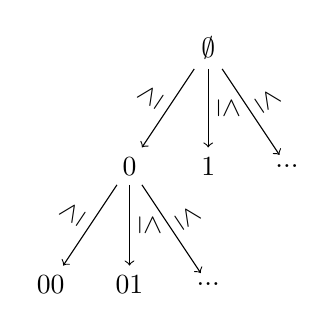
\begin{tikzpicture}
            

            % Root node
            \node (root) at (0,0) {$\emptyset$};
        
            % Second stage nodes
            \node (n1) at (-1,-1.5) {$0$};
            \node (n2) at (0,-1.5) {$1$};
            \node (n3) at (1,-1.5) {$...$};
        
            % Edges
            \draw[->] (root) -- (n1) node[midway, sloped, above] {$\geq$};
            \draw[->] (root) -- (n2) node[midway, sloped, above] {$\leq$};
            \draw[->] (root) -- (n3) node[midway, sloped, above] {$\leq$};
            
            % Third stage nodes
            \node (n00) at (-2,-3) {$00$};
            \node (n01) at (-1,-3) {$01$};
            \node (n02) at (0,-3) {$...$};
        
            % Edges
            \draw[->] (n1) -- (n00) node[midway, sloped, above] {$\geq$};
            \draw[->] (n1) -- (n01) node[midway, sloped, above] {$\leq$};
            \draw[->] (n1) -- (n02) node[midway, sloped, above] {$\leq$};
        
        \end{tikzpicture}
        \hspace{30pt}
        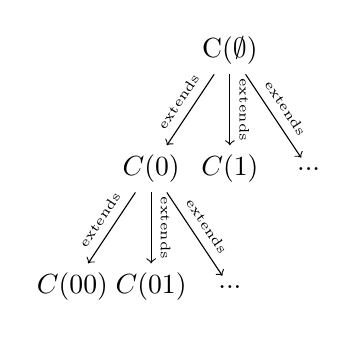
\begin{tikzpicture}
            % Root node
            \node (root) at (0,0) {C($\emptyset$)};
        
            % Second stage nodes
            \node (n1) at (-1,-1.5) {$C(0)$};
            \node (n2) at (0,-1.5) {$C(1)$};
            \node (n3) at (1,-1.5) {$...$};
        
            % Edges
            \draw[->] (root) -- (n1) node[midway, sloped, above] {\tiny{extends}};
            \draw[->] (root) -- (n2) node[midway, sloped, above] {\tiny{extends}};
            \draw[->] (root) -- (n3) node[midway, sloped, above] {\tiny{extends}};
            
            % Third stage nodes
            \node (n00) at (-2,-3) {$C(00)$};
            \node (n01) at (-1,-3) {$C(01)$};
            \node (n02) at (0,-3) {$...$};
        
            % Edges
            \draw[->] (n1) -- (n00) node[midway, sloped, above] {\tiny{extends}};
            \draw[->] (n1) -- (n01) node[midway, sloped, above] {\tiny{extends}};
            \draw[->] (n1) -- (n02) node[midway, sloped, above] {\tiny{extends}};

        \end{tikzpicture}
  

}

    \caption{R and a Kripke frame }
    \label{fig:enter-label}
    
\end{figure}
    \\Also, from now on, the constant elements of our language will be ordered $\{c_0, c_1, c_2 ...\}$


\begin{definition}\textbf{Forcing}.
          When a sentence $\phi$ of a language $\mathcal{L}$ is \textbf{forced} by a structure $C(p)$ of a frame $\mathcal{C}$, we denote:
        $ p \vDash_{\mathcal{C}} \phi$ \\
         Forcing is defined by induction: \cite{book1}

        \begin{itemize}
            \item    $ p \vDash_{\mathcal{C}} \phi                 \Leftrightarrow \phi \text{ is true in } C(p)$ (if $\phi$ is an atomic sentence)\\
            \item    $ p \vDash_{\mathcal{C}} (\phi \to \psi)      \Leftrightarrow$   for all $q \geq p$, if $q \vDash_{\mathcal{C}} \phi$, then $q \vDash_{\mathcal{C}} \psi$
            \item    $ p \vDash_{\mathcal{C}} \neg \phi            \Leftrightarrow $  for all $q \geq p$, q does not force $\phi$\\
            \item    $ p \vDash_{\mathcal{C}} (\forall x) \phi(x)  \Leftrightarrow $  for all $q \geq p$ and $d$ in $\mathcal{L}_{C(q)}$, $q \vDash_{\mathcal{C}} \phi(d)$ \\
            \item    $ p \vDash_{\mathcal{C}} (\exists x) \phi(x)  \Leftrightarrow $  exists a $d$ in  $\mathcal{L}_{C(q)}$, such that $p \vDash_{\mathcal{C}} \phi(d)$\\
            \item    $ p \vDash_{\mathcal{C}} (\phi \land \psi)    \Leftrightarrow p \vDash_{\mathcal{C}} \phi \text{ and } p \vDash_{\mathcal{C}} \psi$ \\
            \item    $ p \vDash_{\mathcal{C}} (\phi \lor \psi)     \Leftrightarrow p \vDash_{\mathcal{C}} \phi$ or $p \vDash_{\mathcal{C}} \psi$ \\

        \end{itemize}
\end{definition}

[TODO extended language ? ] 
\begin{definition}
    \textbf{Truth}
    A sentence is Intuitionistically valid if it is forced in all structures of all Kripke
        frames of that the sentence's language.
\end{definition}

In classical logic, this definition simplifies to the one of forcing, and it's simplified again by the fact that p = q; in fact, we can define classical validity as: \cite{book1}

\begin{definition}
    \textbf{Truth}
    A sentence is classically valid if it is intuitionistically valid in all single-sentenced Kripke frames of that sentence's language. 
\end{definition}

\subsection{Classical tableaux}

\subsubsection{Considerations}
    Here We first define a slightly different version of the destructive tableaux proof tree described by \cite{book1}, where each node is a signed sentence  / truth assertion . This will allow for a more implementation-oriented approach and the translation later on. 
    
    The correspondence of the destructive tableaux proof tree described in \cite{book1} to our new one is shown in figure [TODO].
    
    Generally speaking,
    a node in the usual definition is replaced by a sequence of 
    all nodes in the path that goes from the root to it. Afterwards, some nodes are removed from the newly formed tableaux by adjoining its son(s) and its parent. A node should be removed if its corresponding node in the original tableaux was not a leaf of the atomic tableaux that introduced it.   
    


\subsubsection{Classical tableaux}
The classical tableaux stands on pas mal de defintions, well try to justifiy them briefly:
\begin{definition}
    \textbf{A Signed sentence} is a forcing assertion inside of a tableaux proof. It looks like $T_{q} \phi $ or $F_{p} \phi $ 
    \textbf{A Signed sentence list} is a list forcing assertions inside of a tableau proof. We say that a list of forcing assertions \\$\{ T_{p_1}\phi_{1}, T_{p_2}\phi_{2}, ... F_{p_i}\phi_{i}, F_{p_{i+1}}\phi_{i+1}...\} $
     is "valid" if there exists a frame for witch $ \mathcal{C}(p_1) \vDash \phi_{1}$ and $ \mathcal{C}(p_{2}) \vDash \phi_{2}$ and ... $ \mathcal{C}(p_{i}) \nvDash \phi_{i}$  and $ \mathcal{C}(p_{i+1}) \nvDash \phi_{i+i}$
\end{definition}
 

A Signed sentence list will denote a existance assumption that may or may not be valid. We can infer other assumptions that are, by definition, 
consequences and necessities (?) of a given assumption. The function f, defined bellow, is one of the ways we can do that: 
\begin{definition}
    The function $f$ takes a signed sentence $\sigma$ and a signed sentence list $L$ and returns one or two signed sentence lists. It is defined as follows:
    \\(here we denote $l||l'$ = $l_1,l_2...,l_{|l|}, l'_1,l'_2..,l'_{|l'|} $)
    \begin{itemize}
        \item $f(T \neg \alpha, h||L) = \{L || h || F \alpha\}$.
        \item $f(F \neg \alpha, h||L) = \{L || h || T \alpha\}$.
        \item $f(T (\alpha \land \beta), h||L) = \{L || h || T \alpha || T \beta\}$.
        \item $f(F (\alpha \land \beta), h||L) = \{L || h || F \alpha, L || h || F \beta\}$.
        \item $f(T (\alpha \lor \beta), h||L) = \{L || h || T \alpha, L || h || T \beta\}$.
        \item $f(F (\alpha \lor \beta), h||L) = \{L || h || F \alpha || F \beta\}$.
        \item $f(T (\alpha \to \beta), h||L) = \{L || h || F \alpha, L || h || T \beta\}$.
        \item $f(F (\alpha \to \beta), h||L) = \{L || h || T \alpha || F \beta\}$.
        \item $f(T (\forall x) \phi(x), h||L) = \{L || h || T \phi(c_i) \}$ for the first constant $c_i$ for which $\phi(x)$ is not in L.
        \item $f(F (\forall x) \phi(x), h||L) = \{L || h || F \phi(c_i) \}$ for the first constant $c_i$ not present in $h||L$.
        \item $f(T (\exists x) \phi(x), h||L) = \{L || h || T \phi(c_i) \}$ for the first constant $c_i$ not present in $h||L$.
        \item $f(F (\exists x) \phi(x), h||L) = \{L || h || F \phi(c_i) \}$ for the first constant $c_i$ for which $\phi(x)$ is not in L.
    \end{itemize}
\end{definition}

Of course, this inference must be "well behaved":
\begin{theorem}
    Given a signed sentence list x, x is valid if and only if one of the sentence lists of f(x) is valid 
\end{theorem}
\begin{proof}
    It is truth directly by the definition of forcing. Some special attention must be given to the choice of varibles and structures: 
    When chosing [TODO]
\end{proof}


\begin{definition}
    \textbf{The Tableux development of a sentence } is defined inductivelly: 
    \begin{itemize}
        \item A tree with the single node $\{F \phi \}$ is a tableaux development of $\phi$. 
        \item If $\tau$ is a tableaux development of $\phi$, then $\hookleftarrow(\sigma,\tau)$ is a tableaux development of $\phi$. Where:
    \end{itemize}

    $\hookleftarrow(\sigma,\tau) = $ $\tau$ with $f(\sigma, l) $added to all leaves l that contain $\sigma$

\end{definition}


    % \begin{definition} 
    %     A tree with the single node $\{F \phi \}$ is a tableaux development of $\phi$. \\
    % 
    %     if $\tau$ is a tableaux development of $\phi$ then $\hookleftarrow(\sigma,\tau)$ is a tableaux development of $\phi$.
    % We define the function $\hookleftarrow$: 
    %     
    %     Given a signed sentence $\sigma$ and a tableaux development $\tau$ of $\phi$ :
    %     (here we denote $l||l'$ = $l_1,l_2...,l_{|l|}, l'_1,l'_2..,l'_{|l'|} $)
    %     \begin{itemize}
    %         \item $\hookleftarrow(T \neg \alpha,\tau) = \tau$ with the node $t || h || F \alpha $ 
    %         added to all leaves $h||t$ that contain $T\neg \alpha$.
    %         \item $f(F \neg \alpha,\tau) = \tau$ with $L : \{T \alpha\}$ 
    %         added (adjoined?) to all leaves $L$ that contain $F \neg \alpha$.
    %         \item $f(T (\alpha \land \beta),\tau) = \tau$ with $L : \{T \alpha, T \beta\}$ 
    %         added to all leaves $L$ that contain $T (\alpha \land \beta)$.
    %         \item $f(F (\alpha \land \beta),\tau) = \tau$ with $L : \{F \alpha\}$ and $L : \{F \beta\}$ 
    %         added to all leaves $L$ that contain $F (\alpha \land \beta)$.
    %         \item $f(T (\alpha \lor \beta),\tau) = \tau$ with $L : \{T \alpha\}$ and $L : \{T \beta\}$ 
    %         added to all leaves $L$ that contain $T (\alpha \lor \beta)$.
    %         \item $f(F (\alpha \lor \beta),\tau) = \tau$ with $L : \{F \alpha, F \beta\}$ 
    %         added to all leaves $L$ that contain $F (\alpha \lor \beta)$.
    %         \item $f(T (\alpha \to \beta),\tau) = \tau$ with $L : \{F \alpha\}$ and $L : \{T \beta\}$ 
    %         added to all leaves $L$ that contain $T (\alpha \to \beta)$.
    %         \item $f(F (\alpha \to \beta),\tau) = \tau$ with $L : \{T \alpha, F \beta\}$ 
    %         added to all leaves $L$ that contain $F (\alpha \to \beta)$.
    %      \end{itemize}
    % \end{definition}




\begin{theorem}
    "if there exists a frame that does not force $\phi$ then one of the leaves of $ \hookleftarrow (\sigma_1,\hookleftarrow(\sigma_2(.....(\hookleftarrow(\sigma_n , F\phi)...)))) $ is valid."
\end{theorem}

\begin{proof}

    The proof goes by induction:


             The base case is true by definition. Next we assume $\tau' = \hookleftarrow (\sigma, \tau)$.
             There are two cases to consider:
            \begin{itemize}
                \item If there does not exist a frame that does not force $\phi$, The theorem is valid for $\tau'$.
                \item  If there exists a frame that does not force $\phi$:

                         By the induction hypothesis, there exists a valid leaf $\sigma$ in $\tau$.
                         \begin{itemize}
                    \item If $\sigma$ is a leaf in $\tau$, then the theorem is valid for $\tau'$.
                    \item If $\sigma$ is not a leaf in $\tau$, then:
                         One or two nodes were added to $\sigma$ in $\tau'$ by the definition of $\hookleftarrow$.
                         By the property [TODO] of $f$, one the added nodes are also valid.
                         Consequently, the theorem is valid for $\tau'$.

            \end{itemize}
            \end{itemize}
    \end{proof}

    \begin{theorem}
        If all leaves of $ \hookleftarrow (\sigma_1,\hookleftarrow(\sigma_2(.....(\hookleftarrow(\sigma_n , F\phi)...)))) $ are contradictory, then 
        $\phi$ is intuitionistically valid
    \end{theorem}
    \begin{proof}
    If $\phi$ is not intuitionistically valid, there exists a Kripke frame $\mathcal{C}$ and a world $p$ such that $p \nvDash_{\mathcal{C}} \phi$. By the tableaux development process, at least one leaf remains valid. This contradicts the assumption that all leaves are contradictory. Hence, $\phi$ is intuitionistically valid.   \end{proof}
\begin{figure}
\centering
\makebox[\textwidth][c]{%
\resizebox{0.95\textwidth}{!}{

\begin{tikzpicture}[scale=0.9]
\node {$F \phi$}
    child {node {$\ldots$}
        child {node {$\ldots$}}
        child {node {$T \neg \alpha, ...$}
            child {node {$F \alpha, ... T \neg \alpha$}}}
        child {node {$\ldots$}}
        child {node {$T \neg \alpha, ...$}
            child {node {$F \alpha, ... T \neg \alpha$}}}};
\end{tikzpicture}%



\hspace{0.5cm} \raisebox{1.8cm}{$\hookleftarrow$} 
\hspace{0.5cm}
\raisebox{1.25cm}{
\begin{tikzpicture}[scale=0.9]
\node {$F \phi$}
    child {node {$\ldots$}
        child {node {$\ldots$}}
        child {node {$T \neg \alpha, ...$}}
        child {node {$\ldots$}}
        child {node {$T \neg \alpha, ...$}}};
\end{tikzpicture}
}
%
}%
}
\caption{Example of $\hookleftarrow(T \neg \alpha ,\tau)$ and $\tau$ } 
\label{fig:tree_expansion}
\end{figure}

\subsubsection{Sequent calculus}
    Here we use the multi-conclusion sequent calculus defined by \cite{book2}. 
    We also use a Kripke semantics oriented approach to multi-conclusion sequent calculus, presented in \cite{book3} [TODO].
    
\begin {definition}
    \textbf{Sequent} A sequent is an expression of the form 
    \[
    \Gamma \vdash \Delta
    \]
    where $\Gamma = \{\Gamma_1, \Gamma_2, \Gamma_3,...\}$ and $\Delta = \{\Delta_1,\Delta_2,\Delta_3 ...\}$
     are  finite sets of formulas. $\Gamma $ is called the antecedent, and 
    $\Delta$ is called the succedent. [TODO cite]
\end {definition}


$\Gamma $ represents multiple necessary hipotesis, while $\Delta$ represents multiple possible conclusions. 

\begin {definition}
A sequent is non-valid if there exists a frame  
that forces all sentences in $\Gamma$ and does not force any sentence in $\Delta$. A sequent is valid if not non-valid.
\end {definition}



Not a theorem neither a definition but maybe something:\\

\begin{theorem}
Given a valid signed sentence list $\{ T_{p_1}\phi_{1}, T_{p_2}\phi_{2}, ... F_{p_i}\phi_{i}, F_{p_{i+1}}\phi_{i+1}...\} $ and a frame w, 
if $\{ T_{q_1}\gamma_{1}, T_{q_2}\gamma_{2} , ... F_{s_1}\delta_{1}, F_{s_{2}}\delta_{2}...\}$ is the list obtained by filtering the truth assertions of type T extended by $w$ 
filtering the truth assertions of type F with frames extended by w , then $\gamma_{1}, \gamma_{2}, ... \vdash \delta_1, \delta_2, ...$ is not valid
\end{theorem}
\begin{proof}
A sequence of signed lists $\{ T_{p_1}\phi_{1}, T_{p_2}\phi_{2}, ... F_{p_i}\phi_{i}, F_{p_{i+1}}\phi_{i+1}...\} $ 
inside a tableaux proof signifies an assumption of existance of a frame C 
for witch
 $ \mathcal{C}(p_1) \vDash \phi_{1}$ and $ \mathcal{C}(p_{2}) \vDash \phi_{2}$ and ... $ \mathcal{C}(p_{i}) \nvDash \phi_{i}$  and $ \mathcal{C}(p_{i+1}) \nvDash \phi_{i+i}$
 witch implicitly means, by rules [TODO] of the definition of forcing: 

 ($ \mathcal{C}(p) \vDash \phi_{1}$ for all $p \geq p_1$) and ($ \mathcal{C}(p) \vDash \phi_{2}$ for all $p \geq p_2$) and ... ($ \mathcal{C}(p) \nvDash \phi_{i}$ for all $p \leq p_{i}$) and ($ \mathcal{C}(p) \nvDash \phi_{i+1}$ for all $p \leq p_{i+1}$)
 
 take a structure w inside of $\mathcal{C}$ for witch we can infer: $ w \vDash \gamma_{1}$ and $ w \vDash \gamma_{2}$ and ... $ w \nvDash \delta_1$  and $ w \nvDash \delta_2 ...$.
 w is a counterexample proving the non-validity of 
$\gamma_{1}, \gamma_{2}, ... \vdash \delta_1, \delta_2, ...$
\end{proof}


%
% ---- Bibliography ----
%
% BibTeX users should specify bibliography style 'splncs04'.
% References will then be sorted and formatted in the correct style.
%
% \bibliographystyle{splncs04}
% \bibliography{mybibliography}
%
\begin{thebibliography}{8}

    \bibitem{book1}
    Nerode, A., Shore, R.A.: Logic for Applications. 2nd edn. Texts in Computer Science. Springer, New York, NY (1997). \doi{10.1007/978-1-4612-0649-1}
    
    \bibitem{book2}
    Dummett, M.: Elements of Intuitionism. Oxford Logic Guides. Clarendon Press (2000). \url{https://books.google.fr/books?id=JVFzknbGBVAC}
        \bibitem{kripke1965}
    Kripke, S.A.: Semantical analysis of intuitionistic logic I. In: Studies in Logic and the Foundations of Mathematics. Elsevier (1965)


    \bibitem{book3}
    Svejdar, V.: On Sequent Calculi for Intuitionistic Propositional Logic. CMUC (2005). \url{https://www.muni.cz/en/research/publications/1234567}

\bibitem{ref_article1}
Author, F.: Article title. Journal \textbf{2}(5), 99--110 (2016)

\bibitem{ref_lncs1}
Author, F., Author, S.: Title of a proceedings paper. In: Editor,
F., Editor, S. (eds.) CONFERENCE 2016, LNCS, vol. 9999, pp. 1--13.
Springer, Heidelberg (2016). \doi{10.10007/1234567890}

\bibitem{ref_book1}
Author, F., Author, S., Author, T.: Book title. 2nd edn. Publisher,
Location (1999)

\bibitem{ref_proc1}
Author, A.-B.: Contribution title. In: 9th International Proceedings
on Proceedings, pp. 1--2. Publisher, Location (2010)


\bibitem{ref_url1}
LNCS Homepage, \url{http://www.springer.coBm/lncs}, last accessed 2023/10/25
\end{thebibliography}
\end{document}
